	\سؤال{نصب سیستم‌عامل}

با توجه به صحبت‌های انجام‌شده نیازی به آوردن اسکرین‌شات‌های این قسمت نیست.

\سؤال{دستورات پایه‌ی لینوکس}
\begin{enumerate}
	\item 
		\textbf{دستور \lr{pwd}}
		
		\begin{code}
			> pwd
			
			/home/mostafa/Desktop/University/OS-Lab
		\end{code}
	\item 
		\textbf{دستور \lr{cd} و دستور \lr{mkdir}}
		\begin{code}
			> cd /tmp
			
			> mkdir oslab1
			
			> cd oslab1
		\end{code}
	\item 
		\textbf{دستور \lr{nano}}
		\begin{code}
			> sudo nano information.txt
		\end{code}
	
	\item 
		\textbf{دستور \lr{mv}}
		\begin{code}
			> sudo mv information.txt myinformation.txt
		\end{code}
	\item 
		\textbf{دستور \lr{cp}}
		
		\begin{code}
			> sudo cp information.txt backupinfo.txt
		\end{code}
	\item  
		\textbf{دستور \lr{cat}}
		\begin{code}
			> cat myinformation.txt
		\end{code}
	\item دستور «\lr{>}» تمام محتویات قبلی را پاک کرده و محتوای جدید را به فایل اضافه می‌کند. اصطلاحا به این کار «\lr{overwrite}» می‌گویند.
	 اما دستور «$>>$»، محتوای قبلی را نگه می‌دارد و محتوای جدید را به آخر محتوای قبلی اضافه می‌کند. اصطلاحا به این کار «append» می‌گویند.
	\item 
		\textbf{ساخت فایل جدید با دستور \lr{cat}}
		\begin{code}
			> cat > testfile.txt
		\end{code}
	\item 
		\textbf{لیست پردازه‌ها}
		\begin{code}
			> ps aux
		\end{code}
		\begin{figure}[!htbp]
			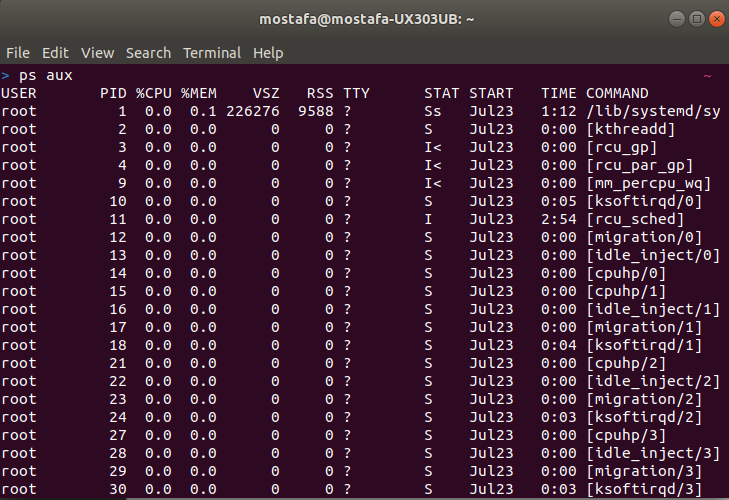
\includegraphics[width=\linewidth]{9.png}
			\caption{نمایش لیست پردازه‌ها با دستور \lr{ps}}
		\end{figure}
	\item 
		\textbf{دستور \lr{grep}}
		\begin{code}
			> ps aux | grep a
		\end{code}
	
	\item 
		\textbf{دستور \lr{ls}}
		\begin{code}
			> cd /usr/bin
			
			> ls
		\end{code}
	
	\item 
		\textbf{نمایش ججم و نام فایل‌ها}
		\begin{code}
			> ls -sh
		\end{code}
	\item 
		\textbf{جست‌وجو در نام فایل‌ها}
		\begin{code}
			> ls -h | grep 'id\textbackslash|fs'
		\end{code}
 
			
\end{enumerate}